\documentclass[a4paper,timesnewroman,12pt,oneside]{report}
\usepackage[a4paper, margin={2cm}]{geometry}
\usepackage[utf8]{inputenc}
\usepackage{setspace}
\usepackage{graphicx,array}
\usepackage{tabularx}
\usepackage{fancyhdr}
\usepackage[sf,bf]{titlesec}
\usepackage{fontspec}
\usepackage{lipsum}
\usepackage{titletoc}
\usepackage[skip=12pt plus1pt, indent=40pt]{parskip}
\usepackage{longtable}
\usepackage{pgffor}
\usepackage{amsmath}
\usepackage{subfigure,float}
\newcommand{\setnumimages}[1]{\def\numimages{#1}}
\allowdisplaybreaks
\fancypagestyle{plain}{}
\renewcommand{\contentsname}{\centering \Huge \vspace{-2cm}  TABLE OF CONTENTS}
\renewcommand\bibname{REFERENCE}
\renewcommand*\listfigurename{\centering \Huge \vspace{-2cm} LIST OF FIGURES}
\renewcommand*\listtablename{\centering \Huge \vspace{-2cm} LIST OF TABLES}
\titlespacing*{\chapter}{0pt}{5pt}{10pt}
%%%%%%%%%%%%%%%%%%%%%%%
\title{Seminar Report-Pothole and Speed Bump Detection}
\author{Anand Ajith}
\date{December 2022}
%%%%%%%%%%%%%%%%%%%%%%%
\begin{document}
\doublespacing
%\maketitle
\pagenumbering{roman}
\thispagestyle{empty}
\graphicspath{{Figures/}}
\begin{center}

    \singlespacing
    \textit{\large Seminar Report On }
    \\
    \huge \textbf{SPEED BUMP AND POTHOLE DETECTION FOR AUTONOMOUS VEHICLES}
    \vspace{10mm}
    \\
    \large \textit{Submitted in partial fulfillment of the requirements for the award of the degree of} \\
    \Large\textbf{Bachelor of Technology } 
    \\in\\
    \textbf{Information Technology} 
    \vspace{10mm}
    \\ \large Submitted by \\
    \textbf{Anand C A \\
   (Uni Reg. No RET19IT011) }\\
   \vspace{8mm}
    Under the guidance of \\
    Dr. Sherly K K\\
    \vspace{8mm}
    \begin{figure}[h]
        \centering
        
\includegraphics[scale=0.5]{rset_logo.png}
        \label{rset_logo}
    \end{figure}
    \vspace{10mm}
    \textbf{Department of Information Technology\\ 
Rajagiri School of Engineering and Technology (Autonomous)\\
Rajagiri Valley, Kakkanad, Kochi, 682039 \\
December 2022 
}

\end{center}   
\thispagestyle{empty}  
\clearpage
\thispagestyle{empty}

\graphicspath{{Figures/}}
\begin{center}
\textbf{
DEPARTMENT OF INFORMATION TECHNOLOGY \\
RAJAGIRI SCHOOL OF ENGINEERING AND TECHNOLOGY (AUTONOMOUS) \\
RAJAGIRI VALLEY, KAKKANAD, KOCHI, 682039 \\
}
    \begin{figure}[h]
        \centering
        
\includegraphics[scale=0.5]{rset_logo_certificate.png}
    \end{figure}

 
\LARGE \textbf{CERTIFICATE} \\
			
								
\end{center}
\noindent
Certified that the seminar work entitled \textbf{“Speed Bump and Pothole Detection for Autonomous Cars”} is a bonafide work done by \textbf{Anand C A}, University Registration Number \textbf{RET19IT023} in partial fulfillment of the award of the Degree of Bachelor of Technology in Information Technology from APJ Abdul Kalam Technological University, Thiruvananthapuram, Kerala during the academic year 2022-2023.

\vspace{4cm}
\begin{center}
   \begin{tabularx}{1 \textwidth} { 
   >{\raggedright\arraybackslash}X 
   >{\centering\arraybackslash}X 
   >{\raggedleft\arraybackslash}X  }
   \textbf{Dr. Sherly k k}
      &  \textbf{Ms. Aiswarya Mohan} & \textbf{Dr. Neeba E.A}\\
     Seminar Guide & Seminar Coordinator & Head of Department\\
     Assoc. Professor & Asst. Professor & Asst. Professor\\
     Dept. of IT & Dept. of IT & Dept. of IT\\
     RSET & RSET & RSET
\end{tabularx} 
\end{center}

			                    		
\addcontentsline{toc}{chapter}{Certificate}
\clearpage


%%%%%%%%%%%%%Header and Footer %%%%%%%%%%%%%%%%%%%%
\fancyhf{} % clear existing header/footer entries
% We don't need to specify the O coordinate

\fancyhead[L]{Speed Bump and Pothole Detection for Autonomous cars}
\fancyhead[R]{RET19IT011} %Registration Number Here
\renewcommand{\footrulewidth}{0.4pt}% default is 0pt
\fancyfoot[L]{Department Of Information Technology}
\fancyfoot[R]{\thepage}
\pagestyle{fancy}
%%%%%%%Acknowledgement and Abstract
\setsansfont[Ligatures=TeX]{Arial}

\begin{center}
    
    \textsf{\Huge \textbf{ACKNOWLEDGEMENT}
    }\\
    
\end{center}
\noindent
I wish to express my sincere gratitude towards Dr. P.S.Sreejith, Principal of Rajagiri School of Engineering and Technology (Autonomous), and Dr. Neeba E.A, Head of Department, Information Technology for providing me the opportunity to present the seminar "Speed Bump and Pothole Detection for Autonomous Cars". I am highly indebted to my seminar coordinators, Ms. Aiswarya Mohan, Assistant Professor, Department of Information Technology, and Ms. Kuttyamma A J,  Professor, Department of Information Technology for their valuable support. It is indeed my pleasure and a moment of satisfaction for me to express my sincere thanks to my seminar guide Dr. Sherly K K , Assistant Professor, Department of Information Technology, for her patience and all priceless advice and for all the wisdom she has shared with me. 
\par \noindent
I would also like to thank the members of my committee, for their valuable feedback and constructive criticism during the preparation of this seminar. Their expertise and guidance have helped me to improve the quality and clarity of my work.
Last but not the least; I would like to express my sincere gratitude towards all other parents, teachers and friends for their continuous support and constructive ideas.
\addcontentsline{toc}{chapter}{Acknowledgement}
\clearpage
%\thispagestyle{empty}
\begin{center}
    \textsf{\Huge \textbf{ABSTRACT}
    }\\
    
\end{center}
\noindent
The development of self-driving cars has always been an extensive research field for the
automobile industry. Many problems must be overcome in order to create a capable self-driving car. Detection of road conditions is one of them. Potholes and speed bumps can cause accidents and have been a concern for drivers. In India, over 10,000 accidents have been reported due to these features. Image processing and acceleration data have been used to try and detect potholes. Detecting potholes and speed bumps can help us take a step toward reducing the number of accidents. Early detection of road irregularities can help to tune the active suspension of the vehicle, thus making the ride comfortable. Speed control of autonomous vehicles is also a major issue. A pothole is a downturn in a street surface; generally, blacktop asphalt, where traffic has eliminated broken bits of the asphalt, and speed humps are parabolic vertical traffic calming systems designed to slow traffic speeds. Hitting a pothole cannot just harm a vehicle's stuns and suspension; it can likewise make the driver lose control of their vehicle. Speed bumps are
useful for keeping vehicle speeds down and encouraging the driver to drive safely.
\par \noindent
The proposed method combines a microcontroller-based speed control system with a camera-based dash cam image retrieval system, as well as an artificial intelligence-based speed bump and pothole detection system to be employed in the construction of self-driving cars. A convolutional neural network model, a deep learning network design that learns directly from data, might be created to recognize potholes and speed bumps, eliminating the human feature extraction requirement. Deep convolutional neural networks (CNNs) have been investigated for many years to help detect potholes. Since the pothole and bumps are identified upfront, we can take preventive measures and make the ride safe and comfortable. The system is extended to send a signal to the speed controller unit of the car to reduce the speed on detection to avoid accidents or damage to the car. The developed car utilizes a single Raspberry Pi as its computational unit. In addition, the research investigates the behavior of economical hardware used to deploy deep learning models. The experimental results indicate that this model can achieve real-time response on a resource-constrained device without significant overheads, thus making it a viable option for autonomous driving in current intelligent transportation systems.
\addcontentsline{toc}{chapter}{Abstract}
    \begin{center}
        \tableofcontents
    \end{center}
    \begin{center}
        \listoffigures
    \end{center}
    \begin{center}
        \listoftables
    \end{center}

%%%%%%%%Chapters From Here

%%%Chapter Styling
\titleformat{\chapter}[display]
  {\normalfont\LARGE\bfseries\sffamily \centering \vspace{-2cm}}{\filcenter\underline{\MakeUppercase{  {\chaptertitlename}}\ \thechapter}}{-20pt}{\underline}

%%%%Section Styling
\titleformat{\section}[block]{\Large\bfseries\sffamily}{\thesection.}{20pt}{\MakeUppercase}
%%%%Subsection Styling
\titleformat{\subsection}[block]{\large\bfseries\sffamily}{\thesubsection.}{20pt}{}
\newcommand{\setupname}[1][\chaptername]{
\titlecontents{chapter}[0pt]{\vspace{1ex}}{\bfseries#1~\thecontentslabel:\quad}{\bfseries}{\bfseries\hfill\contentspage}[]
}
\setupname
\pagenumbering{arabic}
\graphicspath{{Figures/chapter1}}
\chapter{INTRODUCTION}
\section{Genral Background}
specialized development in automobile sector has directed various organizations and institutions to device remote and autonomous vehicles such as intelligent vehicles, unmanned air vehicles (UAV) and drones, which are just the few examples of new generation in the transportation industry. Among all these examples where human is directly involved, safety is the primary concern especially in case of road transportation, as the chances of hazard cannot be ignored. According to the report of world health organization (WHO) estimated number of road traffic death are very high and causes of these situations are random but primarily includes casual driving and inability to understand the scene \cite{R3}. Besides, researchers have started to think on ideas of providing the safety in the form of better scene understanding capability through various sensors.

\noindent
Speed bumps and potholes are common road features that can pose challenges for autonomous vehicles.However, speed bumps and potholes can disrupt the smooth operation of these systems and potentially cause accidents if not properly detected and avoided.To address this issue, researchers and engineers are developing various techniques for detecting and avoiding speed bumps and potholes with autonomous vehicles. These approaches range from simple methods that use sensors to detect changes in road surface height, to more complex methods that employ machine learning algorithms to recognize and classify road features in real-time.
An IVS is expected to regulate its driving speed when it finds such object and ignore the chances of hazard. Understanding the features and detection of speed bump is little explored in existing research studies and had not been associated for the design of IVS \cite{R2}. In addition to the technical challenges, there are also legal and regulatory issues to consider when developing and deploying autonomous vehicles that can detect and avoid speed bumps and potholes. Governments and regulatory bodies around the world are working to establish guidelines and standards for the testing and operation of autonomous vehicles, including requirements for how they should handle road hazards such as speed bumps and potholes.

\noindent
The aim of this seminar is to present a feature descriptor for a speed bump detection model that is suitable for autonomous vehicles. The proposed model is based on a vision-based approach and has been designed to be low-cost and efficient. In addition, we have developed a real-time embedded system prototype to demonstrate the feasibility of implementing the model in autonomous cars. This research aims to contribute a practical solution for detecting speed bumps in real-time, which is a crucial capability for autonomous vehicles to navigate roads safely and efficiently.Our approach combines an artificial intelligence-based speed bump and pothole detection system with a microcontroller-based speed control system. We have chosen to use the Single Shot Multibox Detector (SSD) algorithm, as it is a lightweight algorithm that can run on a feed-forward convolutional network. This is in contrast to the Faster R-CNN algorithm, which uses a regional convolutional network and is not compatible with TensorFlow Lite, which is necessary for running on devices with limited computational power such as the Raspberry Pi \cite{R1}. Our solution aims to provide a practical and effective means for detecting and navigating road hazards in real-time with autonomous vehicles.
\section{Objective}
The goal of this project is to design and develop a system for detecting and safely navigating speed bumps and potholes on the road with autonomous vehicles using a multibox detector algorithm. This system will be designed to enhance the safety and efficiency of autonomous vehicle operation by accurately detecting road hazards and determining the appropriate speed and trajectory to navigate them safely. To achieve this goal, the project will involve implementing the multibox detector algorithm to analyze the detected speed bumps and potholes and determine the appropriate response. The algorithm will be integrated into an autonomous vehicle platform, and the performance of the system will be evaluated through testing on a variety of road surfaces and conditions.
\noindent
In addition to the technical challenges of developing an accurate and reliable system using the single shot multibox detector algorithm, the project will also focus on continually improving the robustness and reliability of the system through ongoing development and optimization. This will involve identifying and addressing potential issues or weaknesses in the system, and testing and refining the system to ensure it performs consistently in a range of real-world scenarios
\section{Relevance}
Accurate detection and safe navigation of speed bumps and potholes is critical for autonomous vehicle operation, as these road hazards can disrupt the smooth operation of the vehicle's sensors and navigation systems and potentially cause accidents if not properly detected and avoided. A system that can detect these obstacles in the road ahead and adjust the speed and trajectory of the vehicle accordingly could greatly improve the safety and efficiency of autonomous vehicle operation, particularly in regions with poor or varied road conditions where these types of obstacles are more likely to be encountered.

\noindent
The proposed project aims to make a significant contribution to the development of autonomous vehicle technology by developing a system for speed bump and pothole detection and speed control. This system could potentially have a major impact on the adoption and deployment of self-driving systems by providing a practical and effective solution for detecting and navigating road hazards in real-time. As such, this project is highly relevant to the seminar, as it addresses an important challenge in the field of autonomous vehicles and presents a potential solution that could have significant practical implications for the deployment and operation of self-driving systems
\clearpage
\graphicspath{{Figures/chapter2}}
\chapter{LITERATURE SURVEY}
This chapter discusses the various related works and previous studies conducted on Speed bump and Pothole Detection. A lot of studies can be seen in recent years for detecting speed bumps and potholes in the road surface automatically.

\noindent
\section{Sensor-based approaches}
 One of the major problems in developing
countries is road maintenance, most of the
accidents happen due to unmarked speed breakers in the
national highway which leads to a threat to drivers. An
Intelligent transportation system plays a vital role in the
advanced driver assistance system. The speed breaker
recognition is used for vehicle and human safety.
Earlier speed breaker detection method involves
sensors, accelerometers, and GPS. Getting into the first sensor-based study approach in this paper,  a novel
method for speed breaker detection and recognition is
developed to alert the driver before the vehicle hit the
speed breaker\cite{R11}. In BLOB analysis, image processing techniques are used to detect the speed breaker in the given image. The camera fixed in the vehicle is used to capture the image of the road and it is analysed in the real-time to detect the presence of speed breaker. This technique can be used for the painted speed breaker. Images captured using a single camera is analysed for finding the speed breakers. This method works fine for colored speed breakers whereas the performance is not up to the mark for uncolored speed breakers. Images taken from more than one camera can be used to improve accuracy. A classification algorithm can also be used for better detection of speed breakers.
\begin{figure}[H]
    \centering
    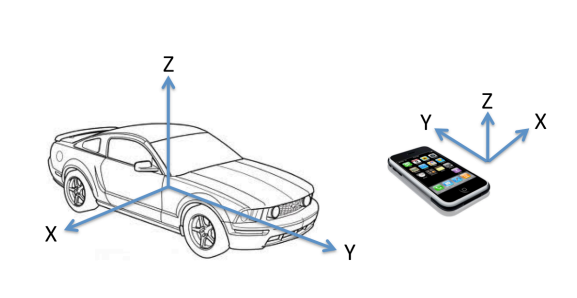
\includegraphics[scale=0.9]{Figures/chapter2/sensor.png}
    \caption{The three axes of a car and a smartphone}
    \label{fig:carsensor}
\end{figure}

\noindent
A system for detecting speed bumps and lanes on roads using HC-SR04 ultrasonic sensor and Wi-Fi sports camera respectively is presented in \cite{R18}. When the speed bump is close to the ultrasonic sensor, the sensor detects the speed bump and the ESP8266 Wi-Fi module transfers the location information to the cloud server through Google Geolocation API. A local database is used to detect the location coordinates of the speed bump.

\noindent
The next paper is the "Road Quality and Ghats
Complexity analysis using Android sensors"\cite{R5} which describes a mobile sensing system (android application) for road irregularity detection using Android OS based smart phone sensors. Selected data processing algorithms are discussed and their evaluation is presented with a true positive rate as high as 90 percent using real-world data. The optimal parameters for the algorithms are determined as well as recommendations for their application.Continuously keeping track on road and traffic conditions in a city is a problem widely studied. Many methods have available towards addressing this problem. But this methods proposed require dedicated hardware such as GPS devices and accelerometers in vehicles or cameras on roadside and near traffic signals. All such proposed are unaffordable to the common man regarding of monetary cost and human effort required. We extend a prior study to improve the algorithm based on using accelerometer, GPS and magnetometer sensor readings for traffic and road conditions detection. This paper explores features and relationships between acceleration data, collected by smartphones, and road roughness conditions. The assumption that a rough estimation of road surface conditions from smartphones would be helpful enough for road management and planning, provided that the approach is very low cost, easy to operate and can be implemented frequently.
\begin{figure}[h]
    \centering
    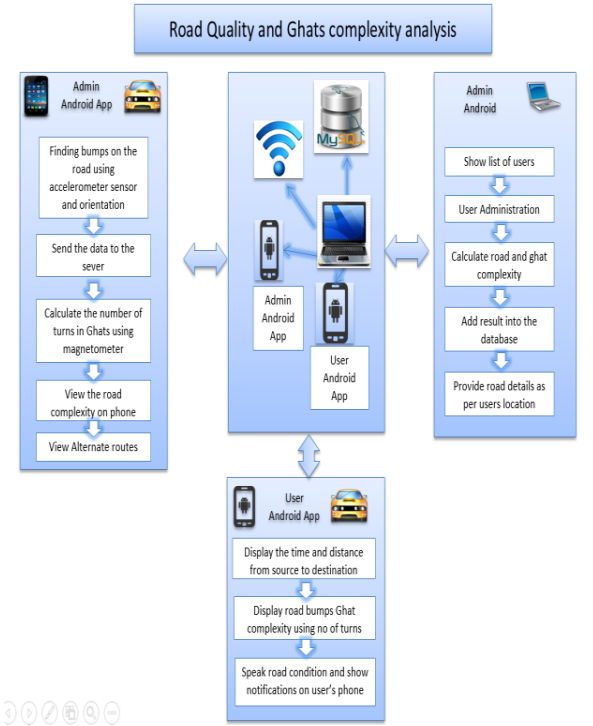
\includegraphics[scale=0.8]{Figures/chapter2/sensor1.png}
    \caption{continuous road condition monitoring system}
    \label{fig:sensor1}
\end{figure}

\noindent
Similarly, scheme of sensor’s signals on speed bump were detected using magnetometer, accelerometer, and GPS. Location and time label of the extracted data were then sent to the server that employed k-means clustering to process the sensor’s data \cite{R10}. In another study of sensors data, Manuel et al. engaged smartphone accelerometer to recognize several road anomalies. It consisted of sliding window method that pre-process the sensors data, then obtained the statistical features, and applied support vector machine (SVM) to classify those anomalies \cite{R6}. In another approach, Jose et al. deployed genetic algorithm (GA) and operated over accelerometer, gyro features, and GPS sensors data to spot speed bumps on the road \cite{R7}. To analyze road conditions; Luis et al. employed machine learning techniques and characterize the accelerometer data by feature pool as Bag of Words (BoW) \cite{R9}. Some of the studies involved smartphone based applications where inbuilt sensors were used to observe the fluctuation patterns of vehicle’s driving through variable road surfaces like speed humps, bumps, uneven roads, cracks, potholes, and smooth road. To counter imminent frontal impacts as an early warning system, smartphone based accelerometer sensors were processed.

\section{Vision-based approaches}
A novel supervision location-aware architecture is proposed for pothole detection \cite{R12}. The approach is based on an intuitive idea: identification of pavement potholes generally first tries to find regions that would more likely contain potholes, then amplifies these areas to a larger resolution and focuses on the discriminative parts to distinguish between areas that have potholes and areas that are pothole free. Such a situation requires tackling the object localization and classification problem as a two-stage process. The proposed approach is to localize the pothole regions under supervision of the center of each pothole. However, to obtain better classification results, it may be beneficial to fnd candidate object parts and focus on the discriminative regions instead of directly running the experiments on the whole image to be classified.More details of potholes are detected in the high-resolution than the low-resolution.
\begin{figure}[H]
    \centering
    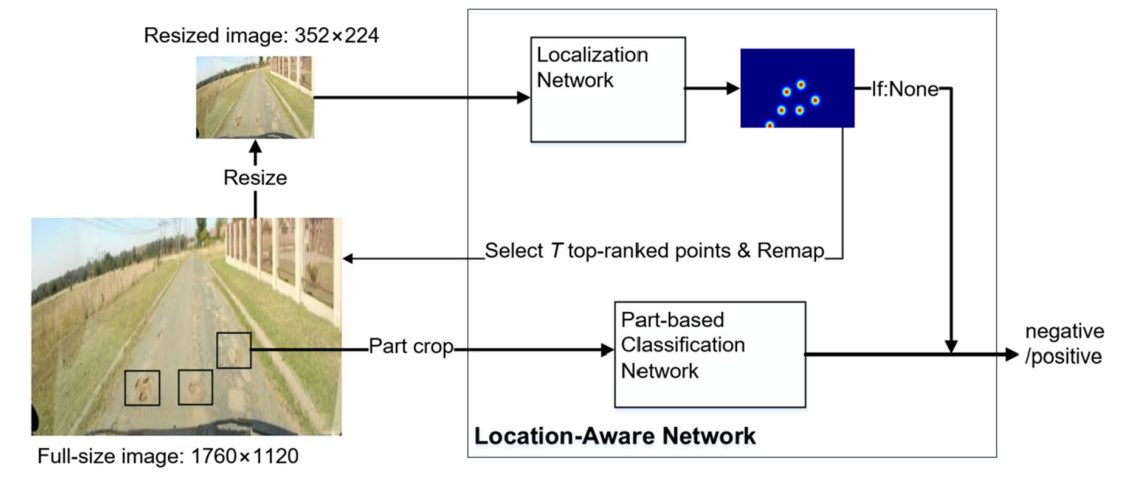
\includegraphics[scale=0.7]{Figures/chapter2/vision1.png}
    \caption{overview of location-aware network approach}
    \label{fig:my_label}
\end{figure}

\noindent
Traditional practices of median and Gaussian filtering,
connected components and binary image conversion had been
applied to recognize speed bumps, mostly to those road areas
where speed bump built with small height example of one such study is the Real Time Speed Bump Detection Using Gaussian Filtering and Connected Component Approach \cite{R13}. The proposed method uses Gaussian filtering and Median filtering to remove noise in the image. Subsequently, image subtraction is achieved by subtracting the Median filtered image from Gaussian filtered image. The resultant image is converted to a binary image and the regions are analyzed using connected component approach. The prior work on speed bump detection is achieved using sensors which are failed to detect speed bumps that are constructed with small height and the detection rate is affected due to erroneous identification. And the smartphone and accelerometer methodologies are not perfectly suitable for real-time scenarios due to GPS error, network overload, real-time delay, accuracy and battery running out. The proposed system goes very well for the roads which are constructed with proper painting irrespective of their dimension.

\noindent
In particular, this methodology suits very well the real time scenario for the painted speed bump though their pattern, color and dimensionality and road condition varies. In addition, it partially identifies illegal speed bumps (speed bumps that falls under category 5). This methodology is robust and effortless to implement in standalone machine that avoids congestion in networking (GPS), saving battery of smartphones while driving. The future scope of the proposed work is detection of bumps in night vision and bad illumination condition like raining and mist.

\noindent
The next paper proposes a method that detects and informs the driver about the upcoming un-marked and marked speed hump/bump in real time using deep learning techniques and gives the distance the vehicle is away from it using stereo-vision approaches. Here they have achieved this using NVIDIA GPU and Stereolab's ZED Stereo camera hardware\cite{R14}. With this driver or autonomous mode of the vehicle can control the vehicle speeds to be at safer limits in order to not cause any kind of discomfort to the passengers as well as damage to the vehicle  This is  achieved by the real-time early detection of marked and un-marked speed humps/bump using deep learning model and distance estimation using ZED stereo camera tested on laptop at 30 frames per second. here by deployed TensorFlow trained deep learning model on to android mobile as app and achieved real-time detection of bump at 2 frames per second. The robust testing of model was carried out on marked and unmarked speed breakers with partially faded paintings, covered by dust, shadows of trees and during night under street lightening conditions. The detection accuracy of proposed model is 97.44\% with false positive rate of 0.0427 for marked speed breakers, accuracy of 93.83\% with false positive rate of 0.0909 for un-marked speed breakers. The distance towards speed breaker is estimated with an accuracy of ±20cm in range of 2-10m. ZED camera doesn’t use IR, but uses color images for depth perception. So the detection of hump is poor at very lowlight environments. It was observed speed hump detection capabilities of the model were becoming low above 14m onwards as the object becomes smaller in the frame captured from the road scene. By use of models like faster RCNN which need little higher computational power but performs exceptionally well on smaller object detections, the distance estimation and can be improved till 20m with ZED camera.

\begin{figure}[h]
    \centering
    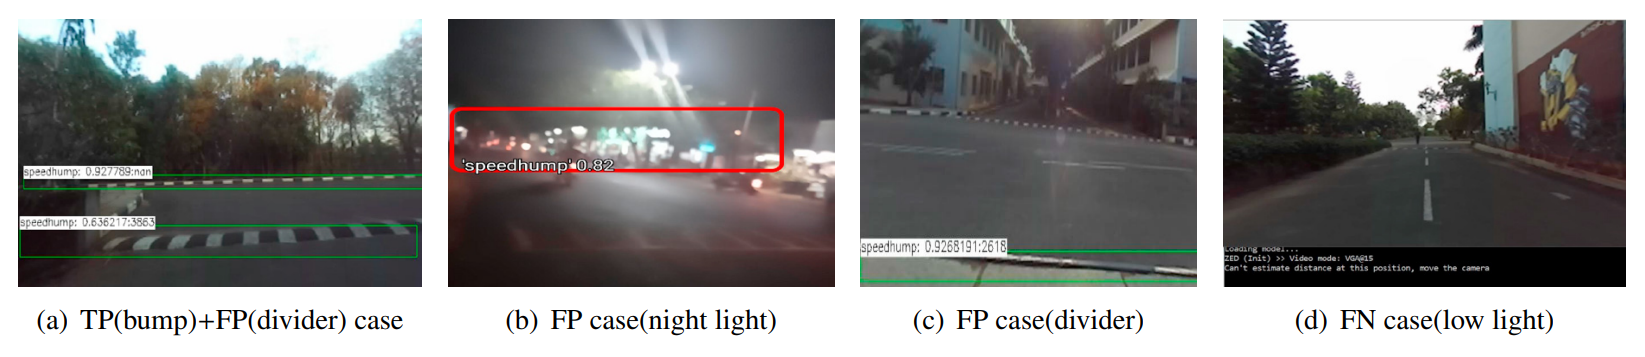
\includegraphics[scale=0.48]{Figures/chapter2/literature_results1.png}
    \caption{ Results of hump/bump detection and distance estimation}
    \label{fig:lit_res}
\end{figure}


\noindent
The next related study is Pothole and Bump detection using Convolution Neural Networks.In this paper an attempt to identify the road surface by classifying it into potholes, speed bump and normal roads based on image data\cite{R8}. The method of classifying the road surface from the images using convolution neural networks, ResNet-50 is discussed. Initially the images are manually classified into three classes and these are used to train the neural network, we were able to achieve a true positive rate of 88.9\%. In the second phase we pass the image to object detection neural network to detect the precise location of the speed bump. This was achieved using the YOLO algorithm for object detection. This work can be extended to alert the driver and tune the suspension to make the ride more comfortable based on road preview using a camera.Machine Learning based approaches can be used to detect pothole and speed bumps using images as opposed to sensor-based methods like accelerometers. This approach makes the method independent of the vehicle platform and can be easily implemented on any vehicle. Since the pothole and bumps are identified upfront, we can take preventive measures and make the ride safe and comfortable. It will be beneficial to consider more input images to cover a wide range of scenarios like rains, low light conditions, different road surfaces, etc. 

\noindent
The main limitation in this paper was that the
network can be made more robust by giving more input images,
training it for a longer time, and tuning the hyper-parameters. The number of input images used during the study did not cover a wide range of scenarios like rains ,low light conditions , different road surfaces etc.The next one was here was the data collection. To make the network more robust we need to gather more data and label the same which was not done.


\noindent
 In this paper,  an efficient pothole detection system is proposed using deep learning algorithms which can detect potholes on the road automatically\cite{R15}. Four models are trained and tested with preprocessed dataset, including YOLO V3, SSD, HOG with SVM and Faster R-CNN. In the phase one, initial images with potholes and non-potholes are collected and labeled. In the phase two, the four models are trained and tested for the accuracy and loss comparison with the processed image dataset. Finally, the accuracy and performance of all four models are analyzed. The experimental results show that the YOLO V3 model performs best for its faster and more reliable detection results. 

\begin{table}[h]
\begin{center}
  \begin{tabular}{|l|l|l|l|l|}
\hline
\textbf{Size} & \textbf{YOLOv3} & \textbf{SSD} & \textbf{HOG} & \textbf{Faster-RCNN} \\ \hline
200 images    & 53\%            & 47\%         & 24\%         & 72\%                 \\ \hline
650 images    & 67\%            & 59\%         & 25\%         & 71\%                 \\ \hline
850 images    & 65\%            & 55\%         & 27\%         & 67\%                 \\ \hline
1000 images   & 69\%            & 59\%         &              & 69\%                 \\ \hline
1100 images   & 73\%            &              &              & 60\%                 \\ \hline
1500 images   & 82\%            & 80\%         &              & 74\%                 \\ \hline
\end{tabular}  
\end{center}

\caption{Comparison of accuracy of different models}
\label{tab:my-table}
\end{table}

\noindent
Two of the limitations of the study were that they inferred YOLO V3 is the fastest but has the lowest accuracy which is not taken into consideration during the study while comparing the models and If the size of the potholes are large then the performance of the SSD is similar to that of YOLO V3.


\section{3D point cloud-based approaches}
Obtaining significant features of point cloud data consisted
the calculation of height variation, intensity of laser points,determining the z point (in 3D plane), road surface roughness representation and data point intensities in two diverse color spaces. These features were processed and examined the height of data points and the change of slope to the road boundaries\cite{R16}. 
\begin{figure}[H]
    \centering
    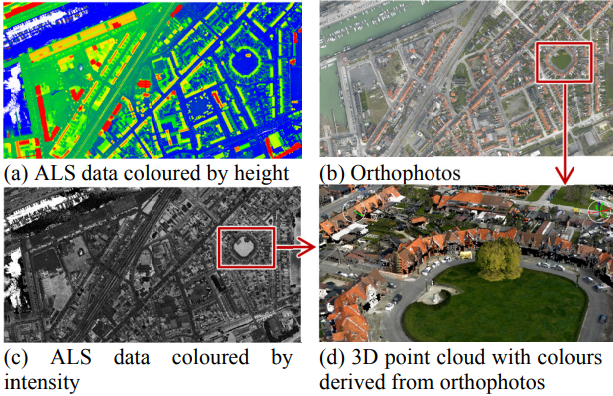
\includegraphics{Figures/chapter2/3dmethod1.png}
    \caption{ALS,Aerial Imagery data and the fusion Results}
    \label{fig:3d1}
\end{figure}

\noindent
This paper presents a workflow including a novel algorithm for road detection from dense LIDAR fused with high-resolution aerial imagery data. Using a supervised machine learning approach point clouds are firstly classified into one of three groups: building, ground, or unassigned. Ground points are further processed by a novel algorithm to extract a road network. The algorithm exploits the high variance of slope and height of the point data in the direction orthogonal to the road boundaries. Applying the proposed approach on a 40 million point dataset successfully extracted a complex road network with an F-measure of 76.9%. 

\noindent
J. Byun et al. applied markov random field (MRF) to differentiate between drivable and non-drivable road area. The computed feature vector formulation is then approximated to the goal region using principal component analysis (PCA) on the neighborhood covariance matrix \cite{R17}. In this paper, a novel method is proposed for road recognition using 3D point clouds based on a Markov random field (MRF) framework in unstructured and complex road environments. The proposed method is focused on finding a solution for an analysis of traversable regions in challenging environments without considering an assumption that has been applied in many past studies; that is, that the surface of a road is ideally flat. The main contributions of this research are as follows: (a) guidelines for the best selection of the gradient value, the average height, the normal vectors, and the intensity value and (b) how to mathematically transform a road recognition problem into a classification problem that is based on MRF modeling in spatial and visual contexts. In the proposed  experiments, they used numerous scans acquired by an HDL-64E sensor mounted on an experimental vehicle. The results show that the proposed method is more robust and reliable than a conventional approach based on a quantity evaluation with ground truth data for a variety of challenging environments. 
\begin{figure}[H]
    \centering
    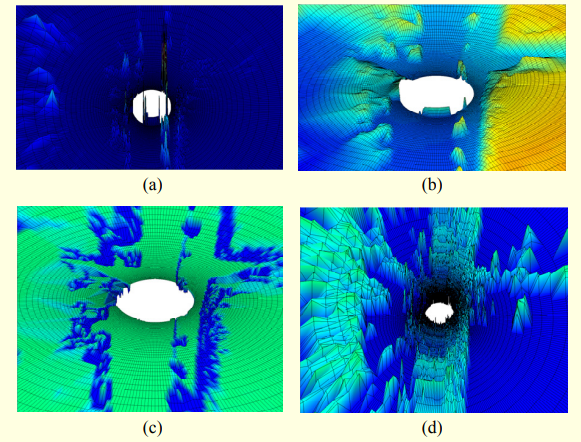
\includegraphics{Figures/chapter2/3dmethod2.png}
    \caption{Display of 3DGI features: (a) gradient value,(b)height value, (c) cosine similarity, and (d) intensity value.}
    \label{fig:3d2}
\end{figure}

\noindent
On the other hand, Suzzane et al. measured dimension of speed bump type of objects using the carrier frequency which was operated with interferometric approach on 24 GHz. This scheme assured a substantial level of sensitivity and appropriate for related types of application \cite{R19}.
This paper shows that an interferometric radar system operating at 24 GHz could be used for
automotive environment awareness in a context of unmanned ground vehicle applications.
The results show that the system can measure the height of small road objects, which tend to
be some number of centimeters high, with good precision using an interferometric technique
allied with SFCW modulation.
The experiments were performed at 24 GHz using two horn antennas for transmitting and
receiving, respectively. We used a vertical linear positioner in order to create many virtual
baselines in the processing, and a horizontal motor rail to measure the targets from different
range positions. Therefore, a model of an automotive scene was created in an indoor
environment. This technique could be used for autonomously driven car applications, as it could
detect small objects on the road and avoid vehicle damage or more serious accidents.




\noindent
As well as 
Surface modelling used the mobile laser scanning (MLS) to yield an even surface and thus the depth representation within reachable and feature-conserving framework got improved \cite{R20}This research work introduces the AGSR algorithm designed to supply scalable and detail-preserving ground surface reconstruction in a fully automatic fashion. 
\noindent
The
proposed technique generates accurate 3D models of outdoor environments adapted for the driving simulator
engine or for being embedded onboard mobile platforms
for autonomous navigation applications.
The reported technique addresses several open issues of
the currently existing surface reconstruction techniques,
such as accurate reconstruction of sharp depth features in
the presence of noisy datasets, scalability, and memory
usage.
Research perspectives of the present research work are
focusing on the photorealist surface reconstruction problem through the joint use of laser reflectance and RGB
cameras. A second research perspective is related to the
facade surface reconstruction and ground–facade merging
within a global referential frame






\section{DeepBus method(ML and IoT) }
This paper proposes a
machine learning based pothole detection system called DeepBus for real time identification of surface irregularities on roads using Internet of Things (IoT)\cite{R21}. DeepBus uses IoT sensors to detect potholes in real time while an end user is driving vehicles on the road. The location of these potholes would be available on a centrally hosted map which can be accessed by both end users and civic authorities. Thus, it would serve as a warning system to all users as well as a database of potholes with thier locations to the authorities for quick repair and action. They have compared the performance of various machine learning models (Logistic Regression, Support Vector Machine (SVM), K-Nearest Neighbors (KNN), Naive Bayes, Decision Tree, Random Forest and Ensemble Voting) based on different parameters (Accuracy, F-score, Precision and Recall) and identified that Random Forest is the best model for pothole detection.Here the live data of these potholes is made available through a real time map for all users to enable smart transportation. With this data, warnings can be given to drivers and their locations shared with civic authorities for quick repair. 





\noindent
Various future improvements can definitely be made to improve and expand the scope of DeepBus. If the system can
differentiate and classify speed bumps it would further add functionality to the DeepBus. Apart from marking potholes,
developing a system to map road conditions would help drivers make more informed choices. Next feature can be added to classify the severity of a pothole. Differentiating a deep pothole with a shallow one will enable Governments to assign priorities while fixing potholes. Another important future direction is reducing misclassifications. A misclassified pothole is detrimental and a waste of time and money to authorities as well as users.

\noindent
 Drawbacks of DeepBus was that the system cannot differentiate and classify speed bumps using the DeepBus method which can be very beneficial.Sensor based approaches may not portray the actual scene effectively, producing a malformed pattern at specific points which are comparatively higher than the actual estimation thus may lead to false detection in given scenario.

\clearpage
\graphicspath{{Figures/chapter3}}
\chapter{METHODOLOGY}
Initially, the proposed approach consist of determining the learning capability of proposed model for speed bump and pothole objects and then speed regulation of the vehicle prototype against the detected speed bump or pothole is followed.  The concept of the integrated system of Figure \ref{fig:units} consists of two units, namely, the detection unit and speed control unit. 
\begin{figure}[h]
    \centering
    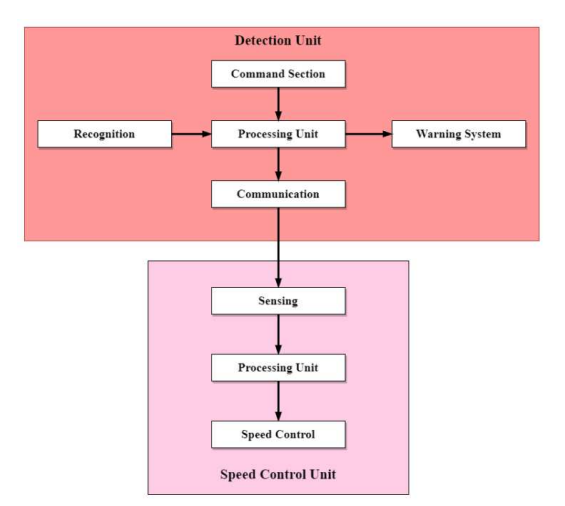
\includegraphics[scale=1]{Figures/chapter3/units.png}
    \caption{Diagram Representation of the System}
    \label{fig:units}
\end{figure}

\noindent
The detection unit deals with object recognition, communication with the speed control unit, warning instructions, and the command section to start, end or modify the system. Contrarily, the speed control unit deals with the sensing of the detection signal sent by the detection unit and controlling the vehicle speed accordingly.

\section{Vehicle Prototype Configuration}
The run-time implementation of the speed bump detection system requires an embedded vehicle prototype. For this purpose, we have chosen the Raspberry Pi 3B+ model(figure \ref{fig:hardware}(a)), which is equipped with a 1.4GHz 64-bit quad-core ARM Cortex-A53 CPU and 1GB LPDDR2 SDRAM module. These resources are sufficient for the operation of the proposed model. The Raspberry Pi 3B+ is also equipped with a monocular camera unit with an 8 megapixel resolution, which is capable of capturing static images of 3280 x 2464 pixels and supports 1080p30 video processing.

\noindent
In addition to the Raspberry Pi 3B+, we have also used a separate Arduino Uno microcontroller(figure \ref{fig:hardware}(b)) module for controlling the wheels and motors of the vehicle.
\begin{figure}[H]
    \centering
        \subfigure[]{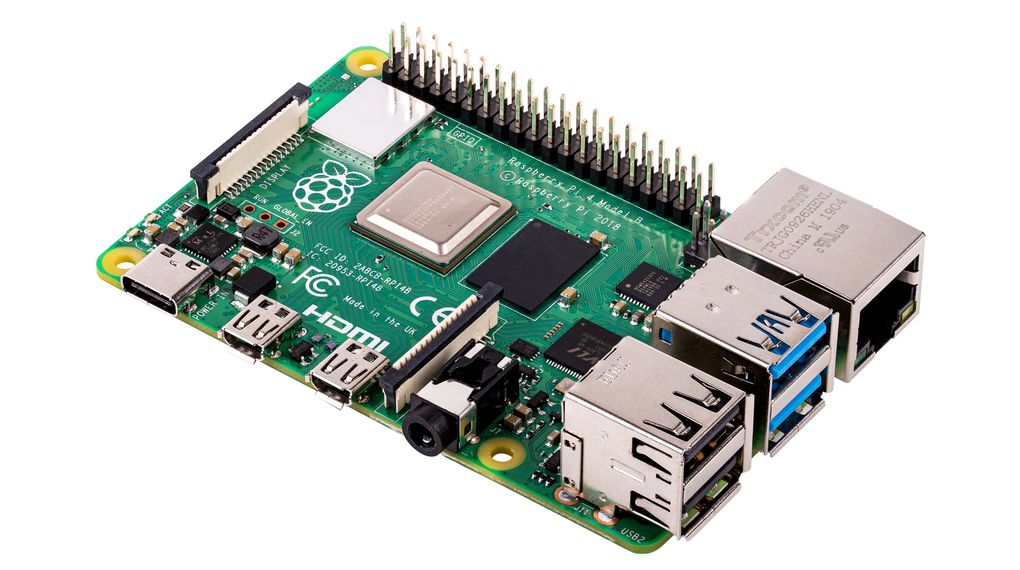
\includegraphics[width=0.45\textwidth]{Figures/chapter3/raspberrypi.jpg}}
        \subfigure[]{ 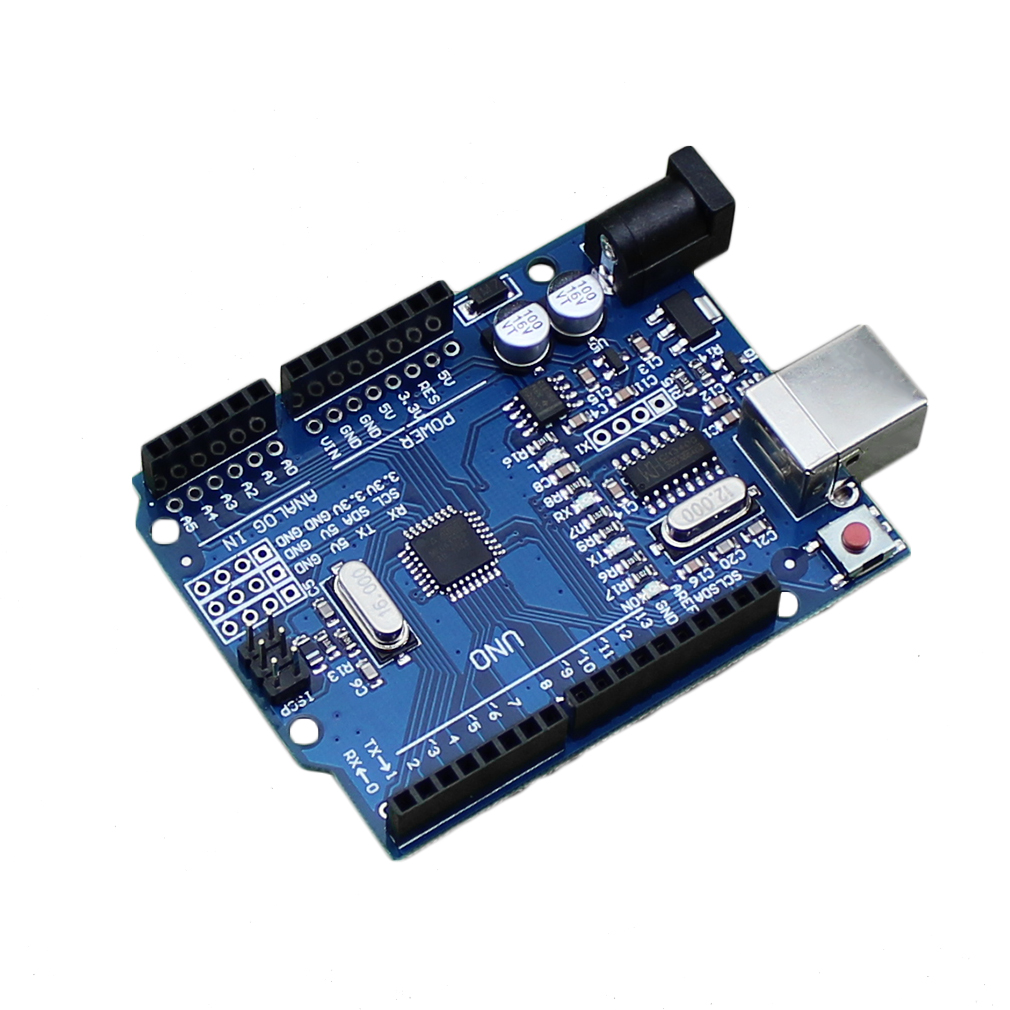
\includegraphics[width=0.45\textwidth]{Figures/chapter3/arduinouno.jpg}}
    \caption{Hardware Components}
    \label{fig:hardware}
\end{figure}

\noindent
\subsection{Hardware Components}
\subsubsection{Raspberry Pi}
The Raspberry Pi is a small, affordable, and versatile single-board computer that is popular among DIY enthusiasts and educators. It was developed in the United Kingdom by the Raspberry Pi Foundation with the goal of promoting the teaching of computer science in schools.

\noindent
One of the main advantages of the Raspberry Pi is its size and low power consumption, which makes it ideal for use in portable or embedded applications. It is also relatively cheap and easy to use, which makes it a popular choice for many projects, including self-driving cars. There are several ways that the Raspberry Pi can be used in a self-driving car project. For example, it can be used as the main computer for running the autonomous driving software, or it can be used to control various subsystems of the car, such as the motors, sensors, and cameras. 

\noindent
The Raspberry Pi is also capable of running a wide range of operating systems and programming languages, which makes it easy to integrate with other hardware and software components. This makes it a flexible platform for building and testing self-driving car prototypes.

\noindent
Overall, the Raspberry Pi is a powerful and cost-effective tool for developing self-driving car technology and other robotics applications. It is a great choice for those who are interested in learning more about autonomous vehicles and exploring the possibilities of this exciting field.
\subsubsection{Arduino UNO}
The Arduino Uno is a microcontroller board based on the ATmega328 microcontroller. It is one of the most popular boards in the Arduino family and is commonly used in a variety of DIY electronics projects, including self-driving cars.One of the main advantages of the Arduino Uno is its simplicity and ease of use. It has a user-friendly design, with a set of digital and analog input/output (I/O) pins that can be easily programmed using the Arduino Integrated Development Environment (IDE). This makes it a great choice for beginners who are just starting out with electronics and programming.

\noindent
In a self-driving car project, the Arduino Uno can be used to control various subsystems of the car, such as the motors, sensors, and cameras. It can also be used to interface with other hardware and software components, such as GPS modules and display screens. The Arduino Uno is also capable of running a wide range of programming languages and libraries, which makes it easy to integrate with other technologies and build complex systems. It is a versatile and powerful platform for developing self-driving car technology and other robotics applications.
\begin{table}[H]
\centering
\begin{tabular}{|l|l|}
\hline
\textbf{Module} & \textbf{Specification}       \\ \hline
Camera          & 8 megapixels, 1080p30,780p60 \\ \hline
DC-motor        & 5v, 20mA, 2000RPM            \\ \hline
Buzzer          & 5v, 20mA                     \\ \hline
H-Bridge        & 5v, 35mA                     \\ \hline
\end{tabular}
\caption{Specification Of Hardware Modules}
\label{tab:hardwarecomp}
\end{table}
\subsection{Serial Communication}
Serial communication is a method of transmitting data serially, or one bit at a time, over a communication channel or computer bus. It is often utilized for transferring data between devices, such as microcontrollers and computers. The Raspberry Pi and Arduino are two popular microcontroller boards that are equipped with serial communication interfaces, allowing for a serial connection to be established between them. To establish a serial connection between the Raspberry Pi and Arduino, a serial cable or wireless serial module must be used to connect the two boards. Additionally, the serial port settings on both boards must be properly configured, including the baud rate and parity. Once the connection is established, serial libraries or terminal programs can be utilized to send and receive data between the boards.

\noindent
Serial communication is a simple and reliable method for exchanging data between the Raspberry Pi and Arduino, and it is frequently employed in various projects, including self-driving cars, robotics, and Internet of Things (IoT) applications. The Raspberry Pi sends a message to the Arduino through the serial port (UART) to request a certain action, such as turning on an LED. The Arduino receives the message and performs the requested action. This process allows for the integration of the Raspberry Pi and the Arduino, allowing for the combination of the Raspberry Pi's advanced computing capabilities with the Arduino's ability to control electronic devices.

\noindent
The Raspberry Pi and Arduino modules are connected using serial communication, allowing the Raspberry Pi to capture frames and identify speed bump objects within bounding boxes. The Raspberry Pi also calculates the distance between the vehicle and the object and sends the processed information to the Arduino, which then modifies the driving behavior of the vehicle accordingly. The developed prototype vehicle can be seen in Figure \ref{fig:carconfig}. 

\noindent
It is equipped with the necessary hardware components, including the Raspberry Pi 3B+ and Arduino Uno, as well as a camera unit and motors for controlling the movement of the vehicle. The prototype is capable of detecting speed bumps and potholes in real-time and adjusting its speed and trajectory accordingly, making it a valuable asset for the safe and efficient operation of autonomous vehicles.
\begin{figure}[H]
    \centering
    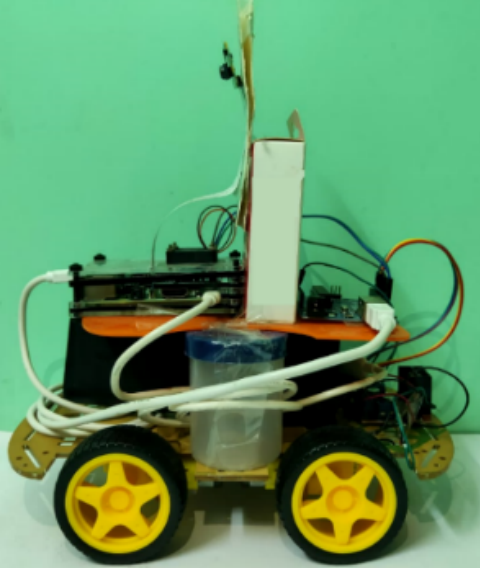
\includegraphics[scale=1]{Figures/chapter3/carconfig.png}
    \caption{Prototype Vehicle}
    \label{fig:carconfig}
\end{figure}


\section{Speed Bump and Pothole Detection}
This section presents an overview of the methods and techniques used in the development of the application for detecting and navigating speed bumps and potholes with autonomous vehicles. The focus of this section is on providing a comprehensive understanding of the steps and techniques involved in the development process.
\noindent
We begin by discussing the creation of the dataset, which is a critical step in any machine learning project. The dataset is used to train and test the network, and it is important that it accurately represents the real-world scenarios in which the system will be used. We also describe the preprocessing techniques applied to the dataset in order to prepare it for use in the network.

\noindent
Next, we describe the training and testing of the network for both classification and detection tasks. Classification involves identifying the type of road hazard (e.g., speed bump or pothole), while detection involves locating and measuring the size and position of the hazard in the road. We describe the specific methods and techniques used to train and test the network for these tasks.

\noindent
Overall, this section aims to provide a thorough understanding of the methods and techniques used in the development of the application for detecting and navigating speed bumps and potholes with autonomous vehicles.
\subsection{Training Data Generation}
The following steps are involved in dataset generation:
\begin{figure}[h]
    \centering
    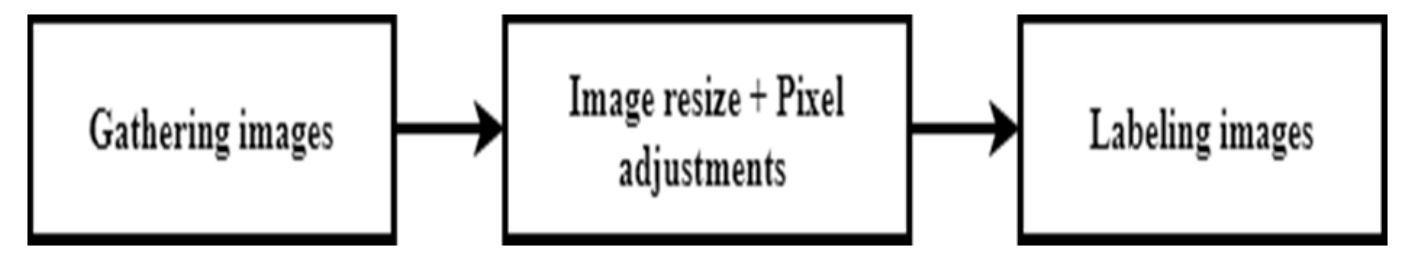
\includegraphics[scale=0.5]{Figures/chapter3/dataset_steps.png}
    \caption{The steps involved in generating training data}
    \label{fig:dataset_steps}
\end{figure}

\noindent
For this Seminar the sample images used in this study were collected from different roads in Rajshahi and Tangail, Bangladesh, totaling approximately 3000 images. Of these, 2500 images were selected for use in training the model, comprising 1000 images of potholes, 900 images of marked speed bumps, and 600 images of unmarked speed bumps. These images were chosen to provide a representative sample of the various road hazards that the model would be expected to encounter in real-world scenarios.

\noindent
The image resolution was carefully considered in the selection process, as the size of the images can have a significant impact on the training time of the model. After evaluating various options, it was determined that a resolution of 800*600 pixels was optimal for this application. This size provided a good balance between image quality and training efficiency.

\noindent
Pixel resizing was also an important consideration in the process of preparing the images for training. If the images are too large, the training time for the model can become prohibitively long. On the other hand, if the images are too small, important details may be lost, which can negatively impact the performance of the model. In this study, the images were resized to a maximum of 200 KB in order to minimize training time without sacrificing image quality.

\noindent
Finally, the software LabelImg was used to construct Extensible Markup Language (XML) files for each image, which contained the necessary annotation data for training the model. These XML files specified the location and dimensions of the road hazards in each image, allowing the model to learn to detect and classify them accurately

\subsection{Training Model}
This study employs the SSD MobileNet v2 Quantized COCO model to develop a learned system for detecting and navigating speed bumps and potholes with autonomous vehicles. The MobileNet model is based on depthwise separable convolutions, which are a type of factorized convolutions that decompose a standard convolution into a depthwise convolution and a 1x1 convolution called a pointwise convolution. This architecture has been designed to be computationally efficient and well-suited for use in resource-constrained environments such as embedded systems.
\subsubsection{Single Shot Multibox Detector}
\noindent
The SSD (Single Shot Multibox Detector) method is a popular approach for object detection tasks, and it uses a feed-forward convolutional network to generate a fixed-size collection of bounding boxes and scores for the presence of object class instances in those boxes. The SSD method uses a CNN architecture that consists of a series of convolutional and max-pooling layers, followed by a series of fully-connected (fc) layers. The convolutional layers are used to extract features from the input image, while the max-pooling layers are used to down-sample the feature maps and reduce the number of parameters in the network. SSD’s architecture(as shown in Figue \ref{fig:ssd_img}) builds on the venerable VGG-16 architecture, but discards the fully connected layers. 
\begin{figure}[h]
    \centering
    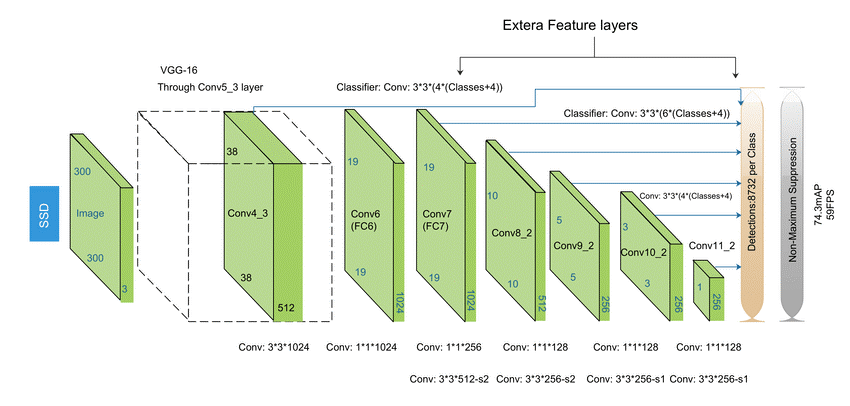
\includegraphics[scale=0.7]{Figures/chapter3/ssd_architecture.png}
    \caption{Single Shot Multibox Detector Architecture}
    \label{fig:ssd_img}
\end{figure}

\noindent
The fc layers are used to make the final predictions for the bounding boxes and class scores. One of the key features of the SSD method is the use of anchor boxes, which are fixed-size bounding boxes that are used as reference points for predicting the locations of object instances in the image. The anchor boxes are defined at multiple scales and aspect ratios, and they are used to predict the locations of object instances at different scales and in different parts of the image.


\noindent
The SSD method also uses a technique called multibox, which involves using multiple sets of fc layers to predict the bounding boxes and class scores for the object instances. Each set of fc layers is responsible for predicting the bounding boxes and class scores for a particular scale and aspect ratio of anchor boxes. This allows the network to make predictions for object instances at different scales and in different parts of the image.This method is known for its efficiency and ability to handle a large number of classes, making it well-suited for applications such as autonomous vehicle obstacle detection.
\subsubsection{MS COCO Dataset}
\noindent
The MS COCO (Microsoft Common Objects in Context) dataset is a large-scale dataset for image segmentation, object detection, keypoint identification, and captioning. It was developed by Microsoft Research and contains 328K images, making it one of the largest and most comprehensive datasets of its kind. The images in the MS COCO dataset are drawn from a wide range of sources, including the Internet and professional image libraries, and they cover a wide variety of object categories and scene types. The dataset is designed to be representative of the types of images that are commonly encountered in real-world applications, and it is widely used as a benchmark for evaluating the performance of object detection and image segmentation algorithms. One of the key features of the MS COCO dataset is the extensive annotation provided for each image. Each image is annotated with a set of bounding boxes that define the location and dimensions of the objects in the image, as well as a set of labels that identify the class of each object. In addition, the dataset also includes annotations for keypoints, which are points of interest on the objects in the image, and captions, which provide a natural language description of the content of the image. 

\begin{figure}[h]
    \centering
    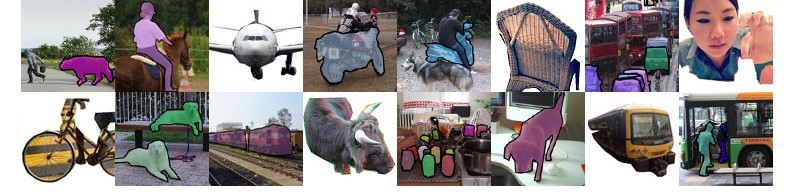
\includegraphics[scale=0.6]{Figures/chapter3/coco-examples.jpg}
    \caption{MS-COCO Dataset Examples}
    \label{fig:coco_eg}
\end{figure}

\noindent
We have chosen the SSD MobileNet v2 Quantized COCO model for this application due to its ability to provide good performance on a Raspberry Pi 4B while still being computationally efficient. The quantized version of the model has been designed to offer minimal model size and fastest performance at the expense of some accuracy compared to the full-precision version of the model.

\noindent
Overall, the combination of the SSD method and the MobileNet v2 Quantized COCO model represents a practical and effective solution for detecting and navigating road hazards in real-time with autonomous vehicles. The combination of efficiency, good performance, and low computational requirements make this model well-suited for use in resource-constrained environments such as autonomous vehicle platforms.

\noindent
SSD implements several enhancements, including multiscale features and default boxes, to make up for the reduction 
in accuracy. The SSD object detection composes of 2 parts: 
\begin{itemize}
    \item Extract feature maps and
    \item Convolutional predictors to detect objects.
\end{itemize}
 VGG16 is used by SSD to extract feature maps.The reason VGG-16 was used as the base network is because of its strong performance in high quality image classification tasks and its popularity for problems where transfer learning helps in improving results. Instead of the original VGG fully connected layers, a set of auxiliary convolutional layers (from conv6 onwards) were added, thus enabling to extract features at multiple scales and progressively decrease the size of the input to each subsequent layer.The architecture of VGG-16 is illustrated in Figure \ref{fig:vgg16}.
 \begin{figure}[h]
     \centering
     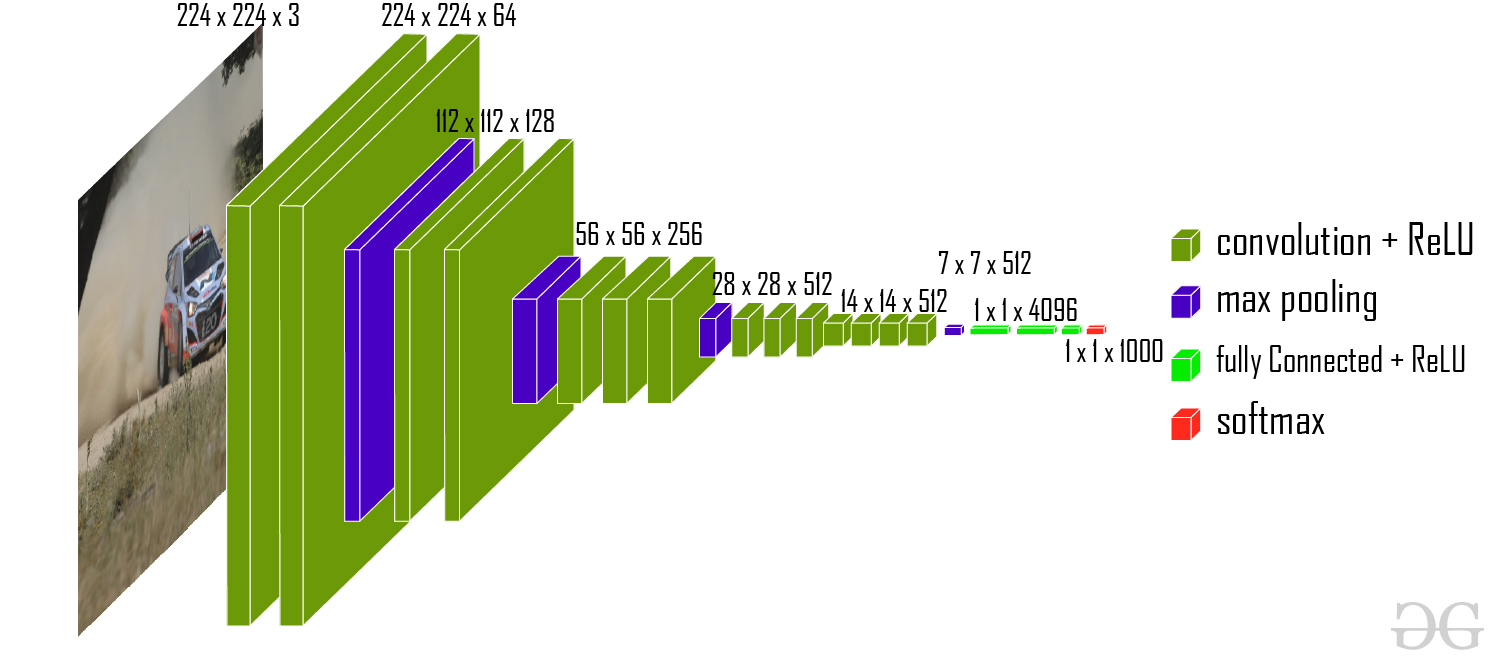
\includegraphics[scale=0.3]{Figures/chapter3/vgg16.jpg}
     \caption{VGG-16 Architecture}
     \label{fig:vgg16}
 \end{figure}

 \noindent
The Conv4\_3 layer is then used to detect objects. SSD calculates both the class scores and the location using small convolution filters. After retrieving the feature maps, SSD uses 3 x 3 convolution filters on each cell for making predictions. Each filter produces 25 channels, with 21 scores for each class and one boundary box for each. For identifying larger-scale objects, SSD employs lower resolution layers. The 4×4 feature maps, for example, are utilized for larger scale objects. Each feature map layer has a scale value defined by SSD. Conv4\_3 detects objects at the smallest size of 0.2 (or 0.1 in some cases) on the left, then grows linearly to the rightmost layer at a scale of 0.9 on the right.

\noindent
Then the width and the height of the default boxes are 
calculated as: 

\begin{flalign}
     w &= scale\sqrt{aspect\ ratio} &\\
    h &= \frac{scale}{\sqrt{aspect\ ratio}} &\\
    SSD\ adds\ an\ extra\ default\ box\ with\ scale: \nonumber &\\
    scale &= \sqrt{scale.aspect\ at\ next\ level} &
\end{flalign}

\noindent
The SSD (Single Shot Multibox Detector) method makes predictions of two types: positive and negative matches. When evaluating the cost of localization (the mismatch between the predicted bounding box and the ground truth bounding box), SSD only considers positive matches. A positive match is defined as a prediction with an intersection over union (IoU) greater than 0.5 between the ground truth bounding box and the associated default bounding box. Conversely, a prediction with an IoU less than 0.5 is considered a negative match. This matching strategy encourages the prediction of shapes that are more closely aligned with the corresponding default bounding box.
\begin{figure}[H]
    \centering
        \subfigure[]{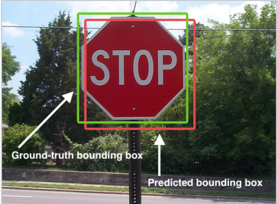
\includegraphics[width=0.45\textwidth]{Figures/chapter3/iou1.png}}
        \subfigure[]{ 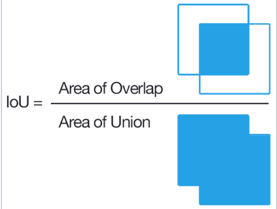
\includegraphics[width=0.45\textwidth]{Figures/chapter3/iou2.png}}
    \caption{IoU Calculation}
    \label{fig:iou_main}
\end{figure}
\begin{figure}[H]
    \centering
    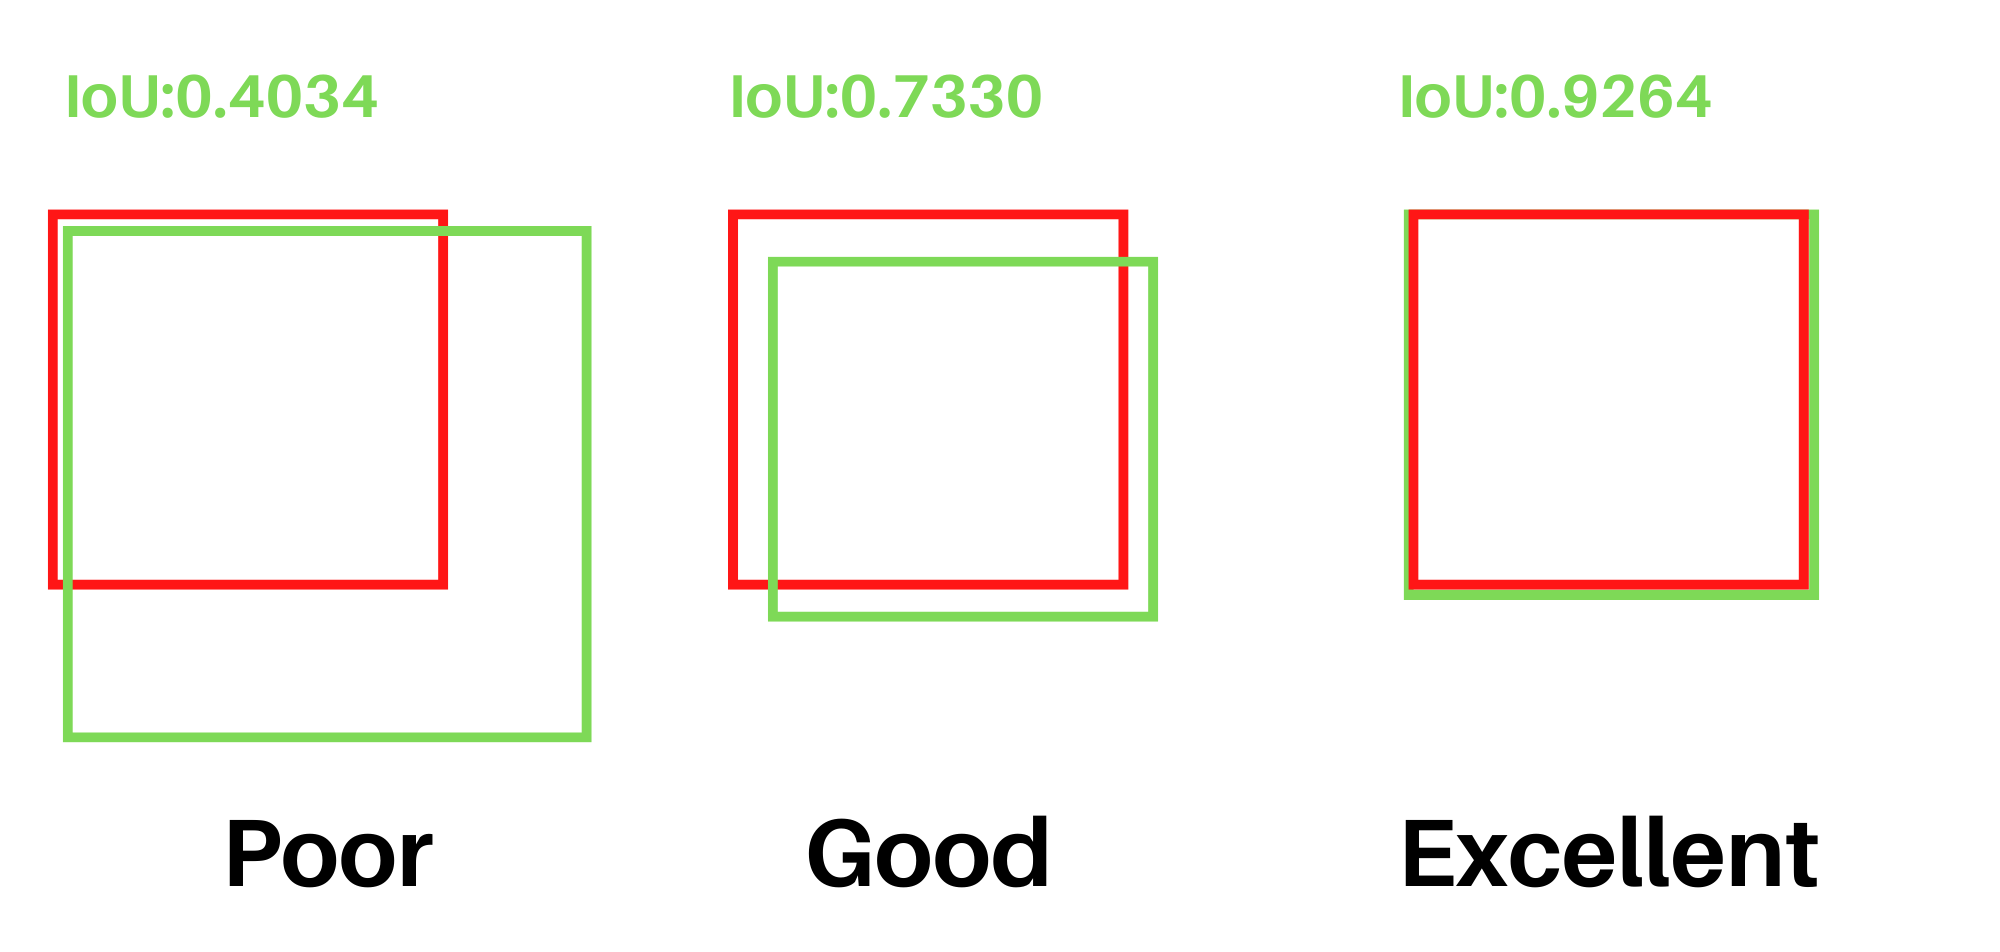
\includegraphics[scale=0.8]{Figures/chapter3/iou3.png}
    \caption{IoU Threshold Ranking}
    \label{fig:iou3}
\end{figure}
\subsection{Loss Function}
The mismatch between the predicted boundary box and the ground truth box is known as the localization loss. It is typically calculated using a measure such as the intersection over union (IoU) between the predicted and ground truth bounding boxes.This matching strategy is used to encourage predictions that are more closely aligned with the corresponding default boxes and to reduce the impact of negative matches on the overall localization loss.By minimizing the localization loss, the SSD method aims to improve the accuracy and precision of the object detection model in predicting the locations and sizes of objects in an image. The localization loss between the predicted box \textit{l} and the ground truth box \textit{g} is defined as the smooth L1 loss with \textit{cx,cy} as the offset to the default bounding box \textit{d} of width \textit{w} and height \textit{h}\cite{R4}.
\begin{flalign}
    l_{loc} &=\sum_{i\in Pos\ m\in\{cx,cy,w,h\}}^{N}\sum\hat{x}_{ij}^ksmooth_{L1}(l_i^m-\hat{g}_j^{m})\nonumber\\
    \hat{g}_j^{cx} &= \frac{ \hat{g}_j^{cx}- \hat{d}_i^{cx}}{ \hat{g}_i^{w}}\\
     \hat{g}_j^{cy} &= \frac{ \hat{g}_j^{cy}- \hat{d}_i^{cy}}{ \hat{d}_i^{h}}\\
      \hat{g}_j^{w} &= \log\log(\frac{ \hat{g}_j^{w}}{ \hat{d}_i^{w}})    \\
      \hat{g}_j^{h} &= \log\log(\frac{ \hat{g}_j^{h}}{ \hat{d}_i^{h}}) \\
        x_{i\ j}^{p} &= \begin{cases}
            1,& \text{if IoU>0.5 between default box i and ground true box j on class p}\\
    0,              & \text{otherwise}   
         \end{cases}        
\end{flalign}
\subsection{Model Implementation}
In order to deploy the trained model on a low-power edge device such as the Raspberry Pi, it is necessary to convert it to a format that is compatible with the TensorFlow Lite framework. TensorFlow Lite is a lightweight version of the TensorFlow framework that is specifically designed for deployment on mobile and embedded devices. Once the trained model has been converted to a TensorFlow Lite file, it can be transferred to the target device and executed using the TensorFlow Lite runtime.
\noindent
In this case, the trained model was converted to a TensorFlow Lite file and transferred to a Raspberry Pi device. The Raspberry Pi is a low-cost, low-power single-board computer that is widely used in a variety of embedded and IoT (Internet of Things) applications. By using the Raspberry Pi camera as the input sensor, the converted model was able to detect the desired object in real-time on the edge device. This allows the model to be deployed in a variety of settings where low-power, low-cost, and real-time performance are key requirements.
\subsection{Object to camera distance calculation}
Once the object is detected that is enclosed in a bounding
box, the very next approach for an IVS is to measure the
distance of this object in real world. Calculating this distance is necessary aspect of IVS; as it has to change its driving behavior according to the detected speed bump. Work in
[41] and [42] involves distance measurement for detected
vehicle object in road environment. The performance under
standard condition was steady but requires high computation.
To overcome this, simple logic is employed to determine the
actual distance of object to the camera. It is obvious that
whenever an object moves away from the camera its size is
reduced and increased when it moves closer to the object.
Using this general perception, the bounding box that holds
speed bump object assist to determine the distance from the
camera and can be visualized in figure \ref{fig:dist_calc}.
\begin{figure}[H]
    \centering
    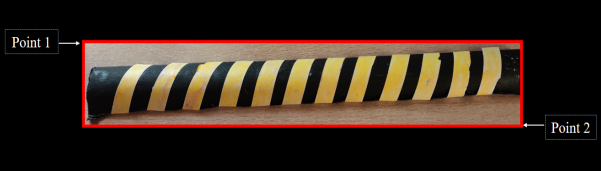
\includegraphics[]{Figures/chapter3/dist_calc.png}
    \caption{Real time detection result}
    \label{fig:dist_calc}
\end{figure}

\noindent
The left and right boundary markings are considered as Point 1 and Point 2. The difference of Point 2 and Point 1 is easily obtainable and measured in pixels. The difference between these two points varies with the scale of object and depends on the vehicle movement towards the speed bump object. It allows to derive the linear equation for calculated difference between Point 2, Point 1 and the tentative distance D1 and D2. For example, the D1 for a random position on track of speed bump to the vehicle position is taken as 60 cm, and let the difference between Point 2 and Point 1 is 70 pixels. Similarly, another distance D2 is set to 90 cm for speed bump to the vehicles fix position and pixel difference between similar points is 45 pixels. Using these parameters we solve equations of y=mx+c for 60=70m+c and 90=45m+c. 

\noindent
Once the parameters of equation is determined, then the
value of m and c will be utilized to calculate the distance
between object and vehicle on every movement (in centimeter)
towards the speed bump. The moment when vehicle comes
closer to object, its size gets increased and is computed with
dynamic change in pixel positions (Point 2 and Point 1). This
helps to represent the actual distance which is closely related to the focal length of camera in real time scenario.

\section{Algorithm And Flowchat}
In the context of this seminar topic, the algorithm is used to detect and classify speed bumps and potholes in the road ahead of an autonomous vehicle. The algorithm begins by collecting input images from the front-facing camera of the raspberry pi as it drives along the road. The input images are then processed by a Single Shot Multibox Detector (SSD) trained to detect and classify speed bumps and potholes. The SSD generates a set of bounding boxes and scores for the detected objects, which are then passed through a non-maximum suppression step to generate the final set of detections. Based on the location and size of the detected speed bumps and potholes, the algorithm calculates the appropriate speed and trajectory to safely navigate the obstacles. It also includes mechanisms to handle false positives and false negatives, as well as to update and refine the model based on new data.The algorithm is designed to enable the autonomous vehicle to detect and safely navigate speed bumps and potholes in real-time, improving the safety and efficiency. The general algorithm for the project is given below: 

\noindent
Step 1: Power supply to the components. \\
Step 2: The python script for detection is initialized on the Raspberry Pi \\
Step 3: Script checks the video feed for speedbump or pothole \\
Step 4: If detected, it blinks the LED, turns on the buzzer, and sends the signal to Arduino.\\ 
Step 5: Arduino slows down the motors to a predetermined value. \\
Step 6: Arduino checks if the detection signal still 
available or not. \\
Step 7: If available, it maintains the reduced speed. \\
Step 8: Else it speeds up to the initial speed. \\
Step 9: Raspberry Pi turns off the LED \& Buzzer. \\
Step 10: Step 3 to step 9 is repeated until the device is turned off. \\
Step 11: Cut the power supply to end the process.

\noindent
To illustrate a procedure or a program, a flowchart is the graphical or pictorial representation of an algorithm using numerous symbols, shapes, and arrows. The flowchart-based on the algorithm of the proposed system is given below: 
\begin{figure}[h]
    \centering
    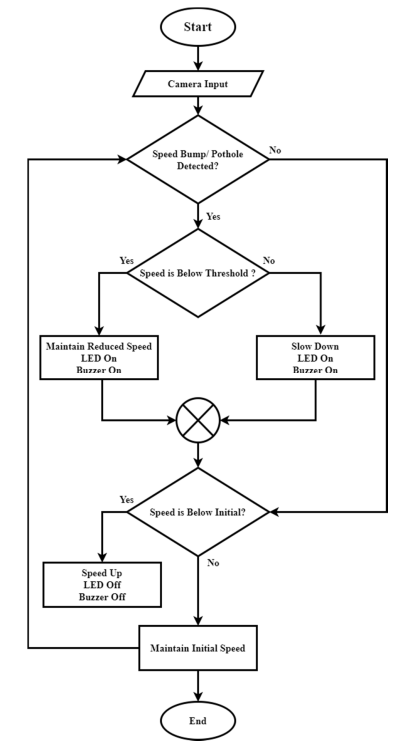
\includegraphics[scale=1]{Figures/chapter3/flowchart.png}
    \caption{Flow Chart of Proposed System}
    \label{fig:flowchart}
\end{figure}
\clearpage
\graphicspath{{Figures/chapter4}}
\chapter{RESULTS AND DISCUSSION}
\section{Loss Function}
In the context of this project, the object detection model is trained using a multi-loss objective function that includes several different loss terms. These include:
\begin{itemize}
\item Classification loss: This loss measures the discrepancy between the predicted class probabilities and the ground truth class labels for a given image. It is typically calculated using a cross-entropy loss function, which penalizes the model for predicting incorrect class labels and rewards the model for predicting correct class labels.

\item Localization loss: This loss measures the discrepancy between the predicted bounding boxes and the ground truth bounding boxes for a given image. It is typically calculated using a measure such as the intersection over union (IoU) between the predicted and ground truth bounding boxes.

\item Regularization loss: This loss term is used to prevent overfitting of the model to the training data. It is typically calculated using a measure such as the L2 norm of the model parameters, which penalizes large parameter values and encourages small parameter values.

\item Clone loss: This loss term is used to fine-tune the model by forcing it to make predictions that are similar to those of a pre-trained model. It is typically calculated using a measure such as the cosine similarity between the predicted class probabilities and the class probabilities of the pre-trained model.

\item Total loss: This is the sum of all the individual loss terms, including the classification loss, localization loss, regularization loss, and clone loss (if applicable). The total loss is used to evaluate the overall performance of the model and to guide the optimization process. By minimizing the total loss, the model can learn to improve its predictions and reduce the overall error.
\end{itemize}
Figures \ref{fig:loss_func}(a), \ref{fig:loss_func}(b), \ref{fig:loss_func}(c), \ref{fig:loss_func}(d), and \ref{fig:loss_func}(e) demonstrate the reduction in loss over time during the training process of the object detection model. As the model learns to better fit the training data, the loss decreases towards zero, indicating that the model is improving in its ability to predict the locations and sizes of speed bumps and pothole.
\begin{figure}[H]
    \centering
    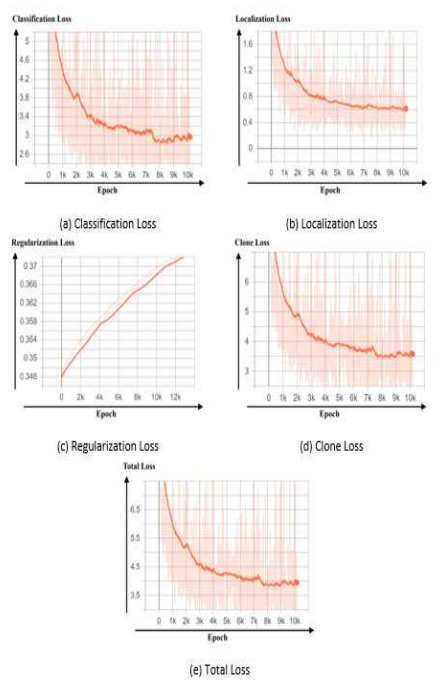
\includegraphics{Figures/chapter4/loss_function.png}
    \caption{Evolution of loss}
    \label{fig:loss_func}
\end{figure}
\section{Real Time Detection Result}
Figure \ref{fig:results} illustrates the real-time detection of speed bumps and potholes by the proposed model. Figures \ref{fig:results}(a) and \ref{fig:results}(b) show the recognition of marked speed bumps with accuracy rates of 90\% and 92\%, respectively. Figure \ref{fig:results}(c) shows the detection of an unmarked speed bump with an accuracy rate of 79\%. Figures \ref{fig:results}(d) and \ref{fig:results}(e) demonstrate the detection of potholes with accuracy rates of 93\% and 67\%, respectively. These results indicate that the trained model is relatively accurate and can be applied in real-world scenarios. It is able to detect speed bumps and potholes at a distance of up to 50 feet. However, the model has difficulty detecting unmarked speed bumps due to the lack of distinct features, and its ability to detect such obstacles may vary significantly depending on the lighting conditions. The model also performs poorly in the detection of potholes due to the diverse geometries and features of these obstacles. Overall, the detection of marked speed bumps is the most accurate, while the detection of potholes is the least accurate among the different types of obstacles.

\noindent
From the achieved results, it has been observed that the proposed model is capable of extracting significant features from a dynamic road environment and make accurate detection of speed bumps. In addition, our model assist the prototype vehicle to modify its driving behavior according to the detected speed bump which shows the compatibility of model and
hardware interface and can be opted in real-time applications.
\begin{figure}[H]
    \centering
    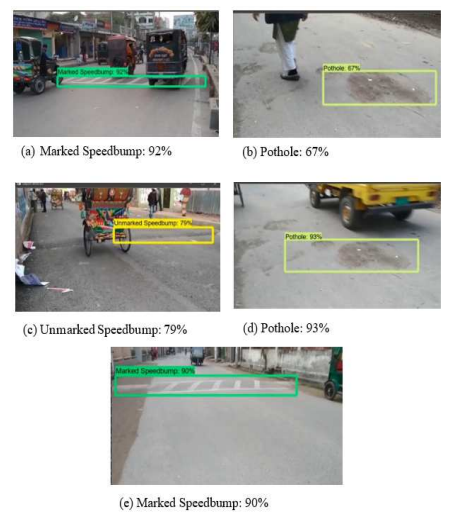
\includegraphics{Figures/chapter4/results.png}
    \caption{Real time detection result }
    \label{fig:results}
\end{figure}
\section{Speed Control Graph}
The performance of the speed bump and pothole detection and speed control system was evaluated through testing on a variety of road surfaces and conditions. Figure \ref{fig:speedtime} shows the graph of time (in milliseconds) versus speed (in RPM) for the system during testing. As can be seen from the graph, the system was able to accurately detect the presence of speed bumps and potholes and adjust the speed of the autonomous vehicle accordingly. The speed of the vehicle decreased from 60 RPM to 30 RPM when a speed bump or pothole was detected, and then gradually increased back to the starting speed of 60 RPM when no obstacles were present. This demonstrates the effectiveness of the system in detecting and safely navigating speed bumps and potholes, and in maintaining a comfortable ride for passengers. Overall, the system showed good performance and accuracy in a variety of road conditions, making it a promising solution for improving the safety and efficiency of autonomous vehicle operation.
\begin{figure}[H]
    \centering
    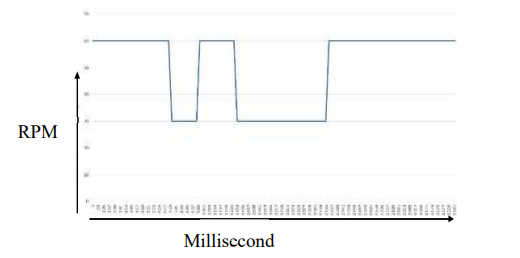
\includegraphics{Figures/chapter4/speedtime.png}
    \caption{Speed vs Time Graph}
    \label{fig:speedtime}
\end{figure}
\clearpage
\graphicspath{{Figures/chapter2}}
\chapter{CONCLUSION}
In this seminar, a real time embedded
system prototype has been proposed, which not only detects
the speed bump using vision camera but also utilizes the
best of its learning through CNN and applies the intelligence
to regulate its speed when such objects occurs. This proposed system can be implemented in
both autonomous and traditional vehicles. In an autonomous
car, it will be capable of controlling the speed of the vehicle
upon detection and for a traditional vehicle, it will warn the
driver about the upcoming speed bump or pothole. A dataset
was created based on the roads of Bangladesh and the data
was trained using the SSD Mobilenet algorithm. The model
was implemented on a Raspberry Pi with a single Raspberry
Pi camera. This system is capable of sending signals to other
devices like Arduino Uno which in turn can control the speed
of motors using a motor driver.Proposed
approach contains two module: first module deals with dataset
preparation, training and detection of speed bump; whereas
second module shows the operational performance over the
detected objects through its logical driving behavior. Test
results have revealed promising outcome and that too with
optimal power depletion


\noindent
 3D detection will be the future work of this system by
using a high-resolution infrared camera and more efficient
and enriched hardware including an enriched dataset and data
augmentation as well as capability
of the prototype is planned to be tested on various cognitive
techniques of optimization.Finally, the adopted strategy and
implementation is not restricted only to speed bump detection
task, but can also be adopted for other intelligent vehicle
applications where the detection of various challenging objects
are required.
\clearpage
%%%%%refs
\bibliographystyle{ieeetr} % We choose the "plain" reference style
\bibliography{IEEEabrv,bibfile} % Entries are in the refs.bib file
\clearpage
%%%%%%%%%%%%%%%%        APPENDIX      %%%%%%%%%%%%%%%%%%%%%%%
\graphicspath{{Figures/slides}}
\setnumimages{28}
\begin{center}
    \LARGE\textbf{\underline{\textsf{APPENDIX-I}}}
    \\
       \LARGE\textbf{\underline{\textsf{SLIDES}}}
    
 
    \vspace{10mm}
    \foreach \x in {1,...,\numimages}{
        \begin{figure}[h]
        \centering
        \frame{\includegraphics[scale=0.6]{slide\x.png}}
        \end{figure}
    }
\end{center}

\addcontentsline{toc}{chapter}{Appendix I}
\clearpage
\addcontentsline{toc}{chapter}{Appendix II}
\begin{center}
    \LARGE\textbf{\underline{\textsf{APPENDIX-II}}}\\
    \vspace{5mm}
    \large\textbf{
  RAJAGIRI SCHOOL OF ENGINEERING AND TECHNOLOGY(AUTONOMOUS)\\\vspace{5mm}DEPARTMENT OF INFORMATION TECHNOLOGY\\PROGRAMME: INFORMATION TECHNOLOGY}

\end{center}
\par \noindent
\textbf{VISION}\\\noindent
To evolve into a department of excellence in information technology through the creation and exchange of knowledge through leading-edge-research, innovation, and services, which will, in turn, contribute towards solving complex societal problems and thus building peaceful and prosperous mankind.
\par \noindent
\textbf{MISSION}\\\noindent
To impart high-quality technical education, research training, professionalism, and strong ethical values to young minds for ensuring their productive careers in industry and academia so as to work with a commitment to the betterment of mankind.
\par \noindent
\textbf{PROGRAMOUTCOMES(PO)}\\\noindent
Information Technology program students will be able to:
\vspace{2mm}
\par \noindent
\textbf{PO 1. Engineering knowledge:} Apply the knowledge of mathematics, science, engineering fundamentals, and an engineering specialization to the solution of complex engineering problems.
\par \noindent
\textbf{PO 2. Problem analysis:} Identify, formulate, review research literature, and analyze complex engineering problems reaching substantiated conclusions using first principles of mathematics, natural sciences, and engineering sciences.
\par \noindent
\textbf{PO 3. Design/development of solutions:} Design solutions for complex engineering problems and design system components or processes that meet the specified needs with appropriate consideration for the public health and safety, and the cultural, societal, and environmental considerations.
\par \noindent
\textbf{PO 4. Conduct investigations of complex problems:} Use research-based knowledge and research methods including design of experiments, analysis and interpretation of data, and synthesis of the information to provide valid conclusions.
\par \noindent
\textbf{PO 5. Modern tool usage:} Create, select, and apply appropriate techniques, resources, and modern engineering and IT tools including prediction and modeling to complex engineering activities with an understanding of the limitations.
\par \noindent
\textbf{PO 6. The engineer and society:} Apply reasoning informed by the contextual knowledge to assess societal, health, safety, legal and cultural issues and the consequent responsibilities relevant to the professional engineering practice.
\par \noindent
\textbf{PO 7. Environment and sustainability:} Understand the impact of the professional engineering solutions in societal and environmental contexts, and demonstrate the knowledge of, and need for sustainable development.
\par \noindent
\textbf{PO 8. Ethics:} Apply ethical principles and commit to professional ethics and responsibilities and norms of the engineering practice.
\par \noindent
\textbf{PO 9. Individual and teamwork:} Function effectively as an individual, and as a member or leader in diverse teams, and in multidisciplinary settings.
\par \noindent
\textbf{PO 10. Communication:} Communicate effectively on complex engineering activities with the engineering community and with society at large, such as, being able to comprehend and write effective reports and design documentation, make effective presentations, and give and receive clear instructions.
\par \noindent
\textbf{PO 11. Project management and finance:} Demonstrate knowledge and understanding of the engineering and management principles and apply these to one’s own work, as a member and leader in a team, to manage projects and in multidisciplinary environments.
\par \noindent
\textbf{PO 12. Life-long learning:} Recognize the need for and have the preparation and ability to engage in independent and life-long learning in the broadest context of technological change.
\par\noindent
\textbf{PROGRAM SPECIFIC OUTCOMES (PSO)}\\\noindent
Information Technology program students will be able to:
\par\noindent
\textbf{PSO1:} Acquire skills to design, analyze and develop algorithms and implement them using high-level programming languages.
\par\noindent
\textbf{PSO2:} Contribute their engineering skills in computing and information engineering domains like network design and administration, database design and knowledge engineering.
\par\noindent
\textbf{PSO3:} Develop strong skills in systematic planning, developing, testing implementing and providing IT solutions for different domains which helps in the betterment of life.
\par\noindent
\textbf{PROGRAM EDUCATIONAL OBJECTIVES (PEO)}\\\noindent
Graduates of Information Technology program shall
\par\noindent
\textbf{PEO 1:} Have strong technical foundation for successful professional careers and to evolve as key-players / entrepreneurs in the field of information technology.
\par\noindent
\textbf{PEO 2:} Excel in analyzing, formulating and solving engineering problems to promote life-long learning, to develop applications, resulting in the betterment of the society.
\par\noindent
\textbf{PEO 3:} Have leadership skills and awareness on professional ethics and codes.
\par\noindent
%%%%%%%%%%tables
\renewcommand{\arraystretch}{2}
\textbf{COURSE OBJECTIVES:}
\vspace{3mm}
\begin{center}
\begin{tabular}{|m{2em}|m{35em}|}
\hline
1 & To do literature survey in a selected area of study.\\
\hline
2 & To understand an academic document from the literate and to give a presentation about it.\\
\hline
3 & To prepare a technical report.\\
\hline
\end{tabular}
\end{center}
\par \noindent
\textbf{COURSE OUTCOMES:}\\
After completion of the course the student will be able to
\vspace{3mm}

\begin{center}
    \begin{tabular}{|m{4em}|m{23em}|m{8em}|}
\hline
\textbf{CO.NO} & 
\textbf{DESCRIPTION} &
\textbf{Blooms' Taxonomy Level}\\
\hline
CO1 & Identify academic documents from the literature which are related to her/his areas of interest.
 & Level 3: Apply\\
 \hline
CO2 & Read and apprehend an academic document from the literature which is related to her/his areas of interest.& Level 4: Analyze\\
\hline
CO3 &Prepare a presentation about an academic document. & Level 6:\\
\hline 
CO4 & Give a presentation about an academic document. & Level 3: Apply\\
 \hline
CO5 & Prepare a technical report.& Level 6:Create\\
\hline
\end{tabular}
\end{center}
\vspace{5mm}
\textbf{CO-PO AND CO-PSO MAPPING}
\begin{center}
\footnotesize
    \begin{longtable}{|m{1.65em}|c|c|c|c|c|c|c|c|c|m{1.3em}|m{1.3em}|m{1.3em}|m{1.3em}|m{1.5em}|m{1.5em}|}
\hline
& PO 1 & PO 2 & PO3 & PO4 & PO5 & PO6 & PO7 & PO8 & PO9 & PO 10 & PO 11& PO 12 & PSO 1 & PSO 2 & PSO 3\\
\hline
CO1 & 2 & 2 & 1 & 1 & & 2 & 1 & & & & & 3 & 1 & &\\\hline
CO2 & 3 & 3 & 2 & 3 & & 2 & 1 & & & & & 3 & 1 & &\\\hline
CO3 & 3 & 2 & & & 3 & & & 1 & & 2 & & 3 & 2 & &\\\hline
CO4 & 3 & & & & 2 & & & 1 & & 3 & & 3 & & & 1\\\hline
CO5 & 3 & 3 & 3 & 3 & 2 & 2 & & 2 & & 3 & & 3 & & & 2\\
\hline
\end{longtable}
\end{center}
\clearpage

\end{document}
